\begin{exercice*}[Pavage]
    \newcommand{\pavageBaseGdeuxExHuit}{%
        \foreach \a in {0,-2,-4}{%
            \draw[shift={(\a,-\a)}] (14,0) -- (14,2) -- (16,2) -- (16,4) -- (12,4) -- (12,0) -- cycle;
            \draw[shift={(\a,-\a)}] (15,2) -- (15,3) -- (13,3) -- (13,1) -- (14,1);
            \draw[shift={(\a,-\a)}] (12,2) -- (13,2);
            \draw[shift={(\a,-\a)}] (14,3) -- (14,4);
            \draw[shift={(\a,-\a)}] (14,0) -- (15,0) -- (15,1) -- (16,1) -- (16,2);
        }
        \foreach \a in {0}{%
            \draw[shift={(\a,-\a)},rotate around={90:(12,0)}] (14,0) -- (14,2) -- (16,2) -- (16,4) -- (12,4) -- (12,0) -- cycle;
            \draw[shift={(\a,-\a)},rotate around={90:(12,0)}] (15,2) -- (15,3) -- (13,3) -- (13,1) -- (14,1);
            \draw[shift={(\a,-\a)},rotate around={90:(12,0)}] (12,2) -- (13,2);
            \draw[shift={(\a,-\a)},rotate around={90:(12,0)}] (14,3) -- (14,4);
            \draw[shift={(\a,-\a)},rotate around={90:(12,0)}] (14,0) -- (15,0) -- (15,1) -- (16,1) -- (16,2);
        }
        \foreach \a in {0}{%
            \draw[shift={(\a,-\a)},rotate around={-90:(16,4)}] (14,0) -- (14,2) -- (16,2) -- (16,4) -- (12,4) -- (12,0) -- cycle;
            \draw[shift={(\a,-\a)},rotate around={-90:(16,4)}] (15,2) -- (15,3) -- (13,3) -- (13,1) -- (14,1);
            \draw[shift={(\a,-\a)},rotate around={-90:(16,4)}] (12,2) -- (13,2);
            \draw[shift={(\a,-\a)},rotate around={-90:(16,4)}] (14,3) -- (14,4);
            \draw[shift={(\a,-\a)},rotate around={-90:(16,4)}] (14,0) -- (15,0) -- (15,1) -- (16,1) -- (16,2);
        }
    }
    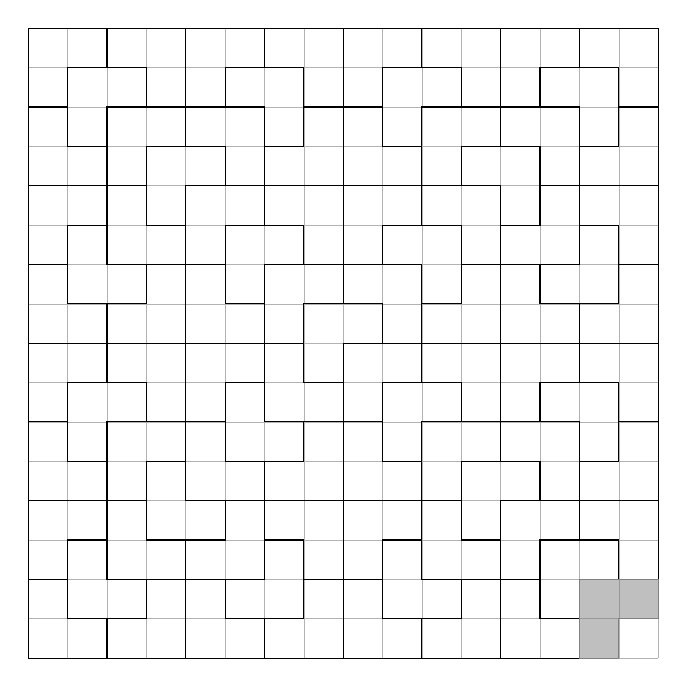
\begin{tikzpicture}[scale=0.5]            
        \draw[help lines, color=black!30] (0,0) grid (16,16);            
        \coordinate (O) at (16,0);
        \tkzDrawPoints[shape=cross out,size=3pt](O);
        \tkzLabelPoints[above](O);
        \pavageBaseGdeuxExHuit
        \begin{scope}[shift={(-8,8)}]
            \pavageBaseGdeuxExHuit
        \end{scope}
        \begin{scope}[rotate around={90:(8,0)}]
            \pavageBaseGdeuxExHuit
        \end{scope}
        \begin{scope}[rotate around={-90:(16,8)}]
            \pavageBaseGdeuxExHuit
        \end{scope}
        \draw[color=gray,fill=gray,fill opacity=0.5] (14,0) -- (15,0) -- (15,1) -- (16,1) -- (16,2) -- (14,2) -- cycle;
    \end{tikzpicture}

\end{exercice*}
\begin{corrige}
    %\setcounter{partie}{0} % Pour s'assurer que le compteur de \partie est à zéro dans les corrigés
    % \phantom{rrr}

\end{corrige}

